%! Author = serox
%! Date = 07/12/2024


\chapter{Introduction}

L'industrie aéronautique est en constante quête de performance, de légèreté et d'efficacité. L'un des enjeux majeurs de cette industrie est la réduction de la consommation de carburant et l'amélioration de l'efficacité énergétique des appareils. Dans ce contexte, les matériaux composites ont émergé comme une solution potentielle aux défis de l'aéronautique moderne. Utilisés pour leur résistance exceptionnelle, leur légèreté et leur durabilité, ces matériaux permettent de réduire significativement le poids des appareils, contribuant ainsi à une diminution de leur consommation de carburant.


\section{Les matériaux composites}

Les matériaux composites sont des matériaux constitués de deux ou plusieurs composants distincts, généralement un renfort et une matrice, qui, lorsqu'ils sont combinés, offrent des propriétés supérieures à celles des matériaux individuels. Dans le domaine aéronautique, ces matériaux sont principalement utilisés sous forme de fibres de carbone ou de verre, intégrées dans une matrice polymère. Les composites offrent des avantages notables, tels que la légèreté et la résistance, ce qui les rend idéaux pour les composants d'avions, les structures de fuselage, les ailes, et d'autres parties essentielles des appareils.


\section{Les avantages des matériaux composites dans l'aéronautique}

L'un des principaux avantages des matériaux composites est leur légèreté, ce qui permet de réduire le poids global de l'appareil. Cela conduit à une meilleure efficacité énergétique, une consommation de carburant réduite et une augmentation de la portée des avions. De plus, leur résistance élevée à la fatigue et à la corrosion permet d'augmenter la durabilité des avions, tout en réduisant les coûts d'entretien à long terme. En outre, les matériaux composites peuvent être moulés dans des formes complexes, permettant des conceptions innovantes et optimisées pour la performance.


\section{Les défis et préoccupations associés aux matériaux composites}

Cependant, l'utilisation des matériaux composites dans l'aéronautique n'est pas sans défis. La fabrication de ces matériaux reste complexe et coûteuse, ce qui a un impact sur le coût global des appareils. De plus, la question du recyclage des composites est encore en développement, car leur dégradation est plus difficile que celle des matériaux métalliques traditionnels. Enfin, bien que les matériaux composites soient généralement résistants, leur comportement en cas de défaillance, notamment lors d'accidents ou de conditions extrêmes, soulève des préoccupations en matière de sécurité.


\section{Problématique}

En conclusion, bien que les matériaux composites offrent de nombreux avantages dans le domaine aéronautique, leur utilisation soulève également des questions importantes. Les avantages qu'ils apportent en termes de légèreté, de résistance et de durabilité doivent être mis en balance avec les défis associés à leur fabrication, leur recyclabilité et leur sécurité. Cela conduit à une question centrale : **les matériaux composites dans l'aéronautique représentent-ils un atout indéniable ou une source de défis potentiellement nuisibles pour l'avenir de l'industrie ?**

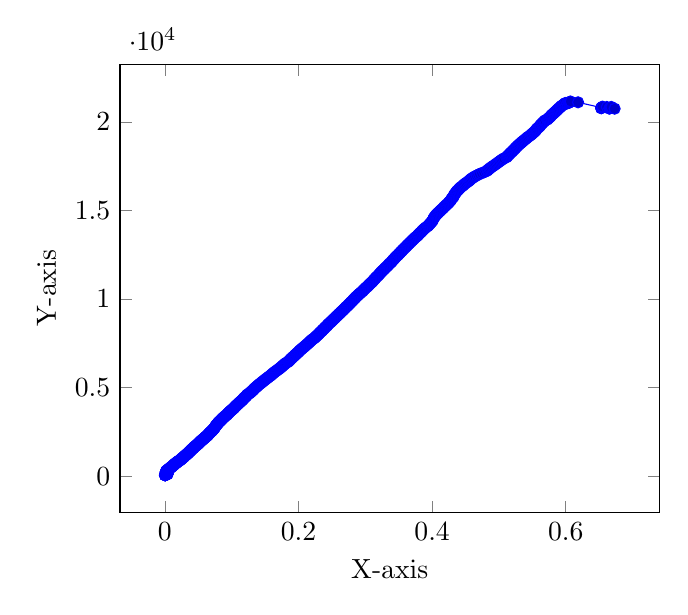
\begin{tikzpicture}
    \begin{axis}[
        xlabel={X-axis},
        ylabel={Y-axis}
    ]
        \addplot coordinates {
            (0,58.1180038452148)
            (0.000181996050429358,57.7992668151855)
            (0.000396029297240692,57.9794960021973)
            (0.0003722525045759,57.9371070861816)
            (0.000237609242728868,58.2010765075684)
            (0.000340537748120779,58.5957221984863)
            (0.000562219820681064,59.5517234802246)
            (0.000412119585783059,61.0890464782715)
            (0.000546498084598015,64.8297729492187)
            (0.000641544969859626,70.6276245117187)
            (0.000887084379853849,76.7926635742187)
            (0.00144146234558031,82.8473510742187)
            (0.0016001323526251,88.3331909179687)
            (0.00220985700861714,93.8126831054687)
            (0.00269316202659016,99.3126831054687)
            (0.0030338178819201,104.660339355469)
            (0.00331101384977411,109.662292480469)
            (0.00354096647022905,113.984558105469)
            (0.00384968242633067,119.234069824219)
            (0.00369128671784479,128.461608886719)
            (0.00403988540617025,135.832366943359)
            (0.00369162130180125,143.340179443359)
            (0.00370719301999114,150.663421630859)
            (0.00341402420418655,158.116546630859)
            (0.00310513527536731,165.639984130859)
            (0.00290711351133105,172.226898193359)
            (0.00262991197867112,178.620452880859)
            (0.00252698532821451,185.816741943359)
            (0.00187748610591387,192.654632568359)
            (0.00153674654662809,199.775726318359)
            (0.001457495362995,207.458343505859)
            (0.00140977634062249,216.269866943359)
            (0.0011325636783507,226.035491943359)
            (0.00129892378345507,236.676116943359)
            (0.00170321748411721,247.197601318359)
            (0.00163977313172449,258.334320068359)
            (0.00239196041342754,269.226898193359)
            (0.00225745534426107,280.101898193359)
            (0.00224155483878757,288.947601318359)
            (0.00224158057601499,293.590179443359)
            (0.00201996496230884,289.156890869141)
            (0.00200386574689029,293.568511962891)
            (0.00274875582901901,302.879058837891)
            (0.00297841768836418,314.238433837891)
            (0.00304179248068279,326.652496337891)
            (0.00382555157288867,340.103668212891)
            (0.00401597204389329,354.117340087891)
            (0.00470526925106081,368.330230712891)
            (0.0050456855878689,382.629058837891)
            (0.00526001965301739,396.634918212891)
            (0.00586980366693934,411.287261962891)
            (0.00632909909786621,425.480621337891)
            (0.00690747534712677,439.410308837891)
            (0.00750135143583398,453.963043212891)
            (0.00794537703929259,467.443511962891)
            (0.00839670691426641,479.636871337891)
            (0.00859499207911663,489.007965087891)
            (0.00868973846485809,496.559722900391)
            (0.00929178183373327,506.284332275391)
            (0.00970372308487633,517.137878417969)
            (0.0100681112144236,529.024963378906)
            (0.0105671630101064,540.821838378906)
            (0.010765205178431,554.323791503906)
            (0.0112721923873681,567.687072753906)
            (0.0116366797559544,581.062072753906)
            (0.0120962288492849,595.773010253906)
            (0.0123650609138281,608.944885253906)
            (0.0129990416313955,621.413635253906)
            (0.0133636440059711,634.075744628906)
            (0.0135455482371026,646.079650878906)
            (0.013870354829547,657.903869628906)
            (0.0139972713583621,669.521057128906)
            (0.0146784091688367,681.239807128906)
            (0.0149000127254633,692.222229003906)
            (0.0152406678851925,703.200744628906)
            (0.0156049716151833,713.909729003906)
            (0.0163965485641182,724.827697753906)
            (0.0165317659284435,736.138244628906)
            (0.0167776264741132,746.439025878906)
            (0.0170232495880633,756.823791503906)
            (0.0173242703450332,767.484130859375)
            (0.0179894186131394,777.866943359375)
            (0.0181006127102707,788.189208984375)
            (0.0185834894700541,797.818115234375)
            (0.0188055419210257,807.521240234375)
            (0.0190667279422229,818.488037109375)
            (0.0194232706228785,828.152099609375)
            (0.0199381413068811,838.764404296875)
            (0.0203421907357497,848.973388671875)
            (0.0209363636141064,858.125732421875)
            (0.0210477190906096,868.055419921875)
            (0.0213878400289697,879.119873046875)
            (0.021997805826552,889.899169921875)
            (0.022631475842455,901.364013671875)
            (0.0229007827704375,912.752685546875)
            (0.023360925443067,923.494873046875)
            (0.0236536787533623,934.959716796875)
            (0.0238909194146485,947.719482421875)
            (0.0244059718823114,959.412841796875)
            (0.0245322966867628,971.229248046875)
            (0.025158645272999,983.697509765625)
            (0.0255625444521075,995.488525390625)
            (0.0259110348585843,1006.66235351562)
            (0.025919014790286,1020.02368164062)
            (0.0265448124607353,1030.64282226562)
            (0.0267663826285264,1040.82641601562)
            (0.0272498585324148,1053.29516601562)
            (0.0278040668295272,1065.77172851562)
            (0.027994427710735,1078.36352539062)
            (0.0285411123902318,1091.93188476562)
            (0.0286361036274341,1103.66821289062)
            (0.0291904250756004,1115.33422851562)
            (0.0293567459951963,1127.82446289062)
            (0.0297210868238932,1140.26196289062)
            (0.0301648949361868,1153.70336914062)
            (0.0304580693167973,1166.57250976562)
            (0.0311155752514282,1179.80297851562)
            (0.0314956960148035,1194.41821289062)
            (0.0319392963743424,1208.57055664062)
            (0.0322085773332305,1222.07250976562)
            (0.0327155237335907,1236.67407226562)
            (0.0333012677859008,1251.20922851562)
            (0.0334919254567582,1266.25219726562)
            (0.034117762080849,1281.77563476562)
            (0.0346407054433188,1295.35571289062)
            (0.0349811194614578,1310.02563476562)
            (0.0351554499917204,1324.89672851562)
            (0.0357492667224977,1340.31079101562)
            (0.0362088121059575,1355.71118164062)
            (0.0365258390997136,1371.79321289062)
            (0.0369298625594879,1386.70141601562)
            (0.0372305216040724,1400.61938476562)
            (0.0377535651330489,1415.83032226562)
            (0.0382367980404118,1430.59204101562)
            (0.0387440115514566,1446.58032226562)
            (0.0389260845817013,1462.96313476562)
            (0.0393617309786328,1477.64086914062)
            (0.0397570214029697,1492.33227539062)
            (0.0400193240952232,1507.66821289062)
            (0.0407004563408919,1523.28149414062)
            (0.0409615162264881,1538.90966796875)
            (0.0414453019045732,1553.74951171875)
            (0.0422768360150113,1569.65966796875)
            (0.0425224220302551,1585.99169921875)
            (0.043226967269401,1601.46044921875)
            (0.043108499970921,1616.88232421875)
            (0.0435363704790348,1632.13623046875)
            (0.0439639108086636,1647.62451171875)
            (0.0445265349472754,1662.58544921875)
            (0.0449703096707334,1677.60888671875)
            (0.0456038776651945,1692.17919921875)
            (0.045872453748665,1706.82763671875)
            (0.0465066783902256,1721.82568359375)
            (0.0470376016843972,1735.59130859375)
            (0.0473463705061551,1750.50537109375)
            (0.0476951985108582,1764.76708984375)
            (0.0483290558752276,1779.59130859375)
            (0.0486697221645686,1794.22998046875)
            (0.0492871633514484,1809.06591796875)
            (0.0494851814056141,1822.71240234375)
            (0.0500636763707344,1836.55163574219)
            (0.050356796958221,1852.08483886719)
            (0.0507607684798065,1866.62390136719)
            (0.0512359101593491,1881.54968261719)
            (0.0515216035858562,1896.02038574219)
            (0.0519172872564787,1909.93054199219)
            (0.0520914471326928,1923.26647949219)
            (0.0527649333350155,1936.53601074219)
            (0.0529946002954328,1950.33483886719)
            (0.0534539935741972,1964.01257324219)
            (0.0538105566591412,1978.66296386719)
            (0.0540877173832243,1992.29382324219)
            (0.0543806747364036,2006.45397949219)
            (0.0550857764561423,2020.33483886719)
            (0.0553230597809407,2033.86218261719)
            (0.0559887144463864,2048.49877929687)
            (0.056567216831248,2062.18627929687)
            (0.0568523723265153,2077.54565429687)
            (0.0572247839787441,2092.44018554687)
            (0.0578425219552734,2105.89135742187)
            (0.0582939724010424,2120.46655273437)
            (0.0590146036391927,2134.16186523437)
            (0.0590069464662349,2148.19506835937)
            (0.0594347910052544,2163.24584960937)
            (0.0599575562939345,2177.44897460937)
            (0.0601950176925225,2191.88256835937)
            (0.060694169654712,2204.42358398437)
            (0.0610902651209732,2217.85913085937)
            (0.0611855939564019,2231.68139648437)
            (0.0620170649990394,2245.81225585937)
            (0.0624528152723482,2261.36889648437)
            (0.0631094920508957,2275.03100585937)
            (0.0632212778723908,2289.83959960937)
            (0.0637759480483952,2305.11303710937)
            (0.0643377708549533,2320.30444335937)
            (0.0646074339305152,2336.14819335937)
            (0.0647421615919188,2351.18725585937)
            (0.0650986801584153,2367.38256835937)
            (0.0655897408927845,2381.82983398437)
            (0.0658667643516547,2397.84545898437)
            (0.0662634830761799,2412.60717773437)
            (0.0668254691170453,2427.34741210937)
            (0.0669523170132539,2443.28881835937)
            (0.0674273882052547,2458.88256835937)
            (0.0680690474275361,2475.98413085937)
            (0.0683940172542877,2492.25366210937)
            (0.0687345165994509,2509.03100585937)
            (0.069566225073808,2524.86694335937)
            (0.0697563782022611,2540.95288085937)
            (0.0704138859918273,2557.45288085937)
            (0.070778165607659,2573.94506835937)
            (0.07092084723167,2591.33959960937)
            (0.0711979523076938,2607.04467773437)
            (0.0719742353150015,2623.04467773437)
            (0.0724184255439688,2638.43920898437)
            (0.0725360432820771,2654.85327148437)
            (0.0731152653818388,2671.38452148437)
            (0.0733607104219992,2689.01342773437)
            (0.0736856950882332,2705.43530273437)
            (0.0741450067498441,2721.97045898437)
            (0.0744459885531725,2737.86206054687)
            (0.0747390089741523,2755.26440429687)
            (0.0748895481041346,2772.89331054687)
            (0.0752856955085844,2791.54565429687)
            (0.0755787530282704,2809.47924804687)
            (0.0759823721121472,2828.27221679687)
            (0.0765054935484067,2846.30346679687)
            (0.0765451669048075,2864.11987304687)
            (0.0769020564583659,2883.04565429687)
            (0.0774007224275043,2900.60815429687)
            (0.0777569961425399,2919.77221679687)
            (0.0784861489535024,2939.36987304687)
            (0.0786761388476483,2958.15502929687)
            (0.0791988225191747,2977.01831054687)
            (0.0794602571017035,2995.73706054687)
            (0.0798322013102342,3014.28784179687)
            (0.0803949961028945,3033.27221679687)
            (0.0808227812839842,3052.87768554687)
            (0.0812030949606316,3072.01049804687)
            (0.0819474953398387,3090.97143554687)
            (0.0824387935059274,3109.4365234375)
            (0.0828822046620648,3127.9951171875)
            (0.0835319439825545,3146.8154296875)
            (0.083991337261319,3165.8505859375)
            (0.0843318662854471,3185.3583984375)
            (0.0850923749228823,3205.8427734375)
            (0.0853457887651325,3224.4599609375)
            (0.0858922749665512,3242.7763671875)
            (0.0865499163114597,3263.1201171875)
            (0.0867162223915732,3281.3583984375)
            (0.0875555435204407,3300.9716796875)
            (0.0881418811520499,3321.1474609375)
            (0.0888550073219378,3340.3583984375)
            (0.0891876417413885,3361.2646484375)
            (0.0898609980982395,3381.5380859375)
            (0.0905105519251983,3401.0888671875)
            (0.0911838192451545,3419.9716796875)
            (0.0918255971832957,3441.2646484375)
            (0.0926968528784525,3461.6435546875)
            (0.0931881584642825,3483.7685546875)
            (0.0934891551070934,3506.01147460937)
            (0.0939557677940827,3526.47631835937)
            (0.0947090496035518,3547.04663085937)
            (0.0953029850501889,3566.85913085937)
            (0.0956833729242488,3588.52709960937)
            (0.0961746562508551,3609.77319335937)
            (0.0968320156455966,3631.04663085937)
            (0.0975369875198637,3652.15209960937)
            (0.0978379915824158,3672.40600585937)
            (0.0987169267097542,3693.27709960937)
            (0.0993747312889699,3714.48803710937)
            (0.0999449977610571,3736.99584960937)
            (0.10082408128322,3759.30834960937)
            (0.101426415876939,3781.33569335937)
            (0.101941026869998,3804.05053710937)
            (0.102813172934104,3825.90600585937)
            (0.103588981077972,3849.02709960937)
            (0.10393765697798,3872.02319335937)
            (0.104222634399458,3895.03100585937)
            (0.105133719265581,3918.16772460937)
            (0.105807416930529,3942.11352539062)
            (0.106139702622142,3966.41430664062)
            (0.106971552071582,3990.23852539062)
            (0.107668814834703,4014.50805664062)
            (0.108191483666747,4037.97680664062)
            (0.109038758758222,4061.73852539062)
            (0.109799289654881,4086.93774414062)
            (0.11048072610994,4110.94580078125)
            (0.111011386003298,4135.27392578125)
            (0.11164508384323,4159.69189453125)
            (0.112651252693322,4182.48876953125)
            (0.113110720169499,4206.10986328125)
            (0.113863185807432,4229.97314453125)
            (0.114576163582495,4254.59423828125)
            (0.115336649960706,4278.49267578125)
            (0.116073244772131,4302.70361328125)
            (0.116516537212408,4326.45361328125)
            (0.117197973667468,4350.50048828125)
            (0.1177051129811,4375.48876953125)
            (0.118544819936512,4400.95361328125)
            (0.11887743951648,4427.27783203125)
            (0.119748628433966,4452.34814453125)
            (0.120438011431891,4478.20361328125)
            (0.121356968643469,4504.65283203125)
            (0.121887346586659,4529.85986328125)
            (0.122481793995442,4556.16845703125)
            (0.122798565008125,4582.28564453125)
            (0.123614506532351,4608.65673828125)
            (0.12474733778512,4634.77001953125)
            (0.126053509032697,4661.32861328125)
            (0.126775108547079,4686.92626953125)
            (0.127480162038499,4712.79345703125)
            (0.128454552136867,4739.19970703125)
            (0.129151429073444,4765.40283203125)
            (0.129872568563869,4792.38720703125)
            (0.130799175528663,4819.76220703125)
            (0.131717976925674,4845.93798828125)
            (0.132217058400322,4872.91064453125)
            (0.13296967243308,4900.61376953125)
            (0.133571725076631,4928.14111328125)
            (0.134403715501155,4955.89013671875)
            (0.135148182658034,4984.11669921875)
            (0.135972011367196,5011.41748046875)
            (0.13685116166703,5038.13232421875)
            (0.137643590031272,5066.45263671875)
            (0.138530634935784,5093.18310546875)
            (0.139179951331023,5120.78857421875)
            (0.140154326589909,5149.42138671875)
            (0.140986124101161,5176.84716796875)
            (0.141881597831719,5204.68310546875)
            (0.142934904297897,5231.95263671875)
            (0.143837961004001,5258.95263671875)
            (0.144637987183271,5286.56982421875)
            (0.145596276443152,5313.67529296875)
            (0.146325800241176,5340.78857421875)
            (0.147402790521387,5368.04638671875)
            (0.148297744870058,5396.31982421875)
            (0.149272105289462,5424.24560546875)
            (0.150151493021015,5451.59326171875)
            (0.150927761188841,5479.28076171875)
            (0.152099872551725,5507.3984375)
            (0.153034923182048,5537.859375)
            (0.154357803686893,5566.4765625)
            (0.155062619746594,5596.1328125)
            (0.15594214103349,5625.15625)
            (0.157281063018892,5652.796875)
            (0.158246890735871,5681.9296875)
            (0.159110697010825,5711.4921875)
            (0.159982012063912,5740.75)
            (0.160750400466542,5769.76171875)
            (0.161788095797155,5799.10546875)
            (0.16254069499043,5827.88671875)
            (0.163625698591177,5856.66015625)
            (0.164520994247946,5886.96484375)
            (0.165669599870588,5916.27734375)
            (0.166865825392496,5946.57421875)
            (0.167760942975475,5976.78515625)
            (0.169084031233075,6007.26953125)
            (0.170184838882659,6037.32421875)
            (0.171040023418294,6067.04296875)
            (0.172188732917313,6098.06494140625)
            (0.173131514918007,6127.92431640625)
            (0.174153628792019,6159.22119140625)
            (0.175183236604682,6190.79931640625)
            (0.17588845333041,6221.26025390625)
            (0.17690264292078,6251.97900390625)
            (0.177821043651764,6282.20556640625)
            (0.178914238646839,6313.68212890625)
            (0.179627275779832,6345.63525390625)
            (0.180894671459697,6377.43994140625)
            (0.182090882142123,6409.54150390625)
            (0.183682327600827,6440.05712890625)
            (0.184974267784708,6470.64306640625)
            (0.185568158712898,6501.74462890625)
            (0.186479035826267,6532.77587890625)
            (0.187358482915751,6565.18994140625)
            (0.187952833867897,6597.89306640625)
            (0.188871249438364,6629.81494140625)
            (0.189687495171981,6660.94775390625)
            (0.190915432667942,6693.90869140625)
            (0.191525305718758,6725.6025390625)
            (0.192562926851959,6758.0791015625)
            (0.193679924376925,6792.3994140625)
            (0.194575576181274,6824.3369140625)
            (0.195106295432561,6857.1728515625)
            (0.196523792477676,6890.3994140625)
            (0.197300164521878,6922.9384765625)
            (0.198100309417008,6955.5791015625)
            (0.199256661249502,6988.2744140625)
            (0.200286372938542,7021.6181640625)
            (0.200911886803889,7054.8134765625)
            (0.201791601004058,7087.8681640625)
            (0.202654843378677,7120.2197265625)
            (0.203874945627891,7151.9619140625)
            (0.20472242847212,7185.2431640625)
            (0.205792266121777,7218.3916015625)
            (0.206869256401987,7253.1572265625)
            (0.208033606715536,7287.2822265625)
            (0.209055646392136,7322.1728515625)
            (0.210085387760141,7355.3056640625)
            (0.211027917489633,7388.2099609375)
            (0.212208249925809,7423.4130859375)
            (0.213150913210642,7458.5771484375)
            (0.21414100348147,7493.0693359375)
            (0.215313367115557,7527.6474609375)
            (0.216176935958791,7562.5927734375)
            (0.217167619808918,7596.5302734375)
            (0.218046562355998,7629.0068359375)
            (0.219092152291288,7664.1083984375)
            (0.220050486069616,7698.6083984375)
            (0.221255036541194,7732.9599609375)
            (0.222545656011135,7768.0068359375)
            (0.224129459136363,7801.7490234375)
            (0.224835106207083,7835.4052734375)
            (0.225785545380734,7870.0224609375)
            (0.226657127544506,7904.7958984375)
            (0.227773887637753,7938.7177734375)
            (0.228827565090993,7975.0615234375)
            (0.229698049133061,8009.2880859375)
            (0.230720904981197,8043.6708984375)
            (0.231568387825426,8079.23681640625)
            (0.232265502193722,8114.33837890625)
            (0.233382366163347,8149.79931640625)
            (0.234515316131976,8186.67431640625)
            (0.235584500844403,8222.884765625)
            (0.236043931221874,8259.126953125)
            (0.237366945282061,8294.939453125)
            (0.238420103353414,8330.400390625)
            (0.239149285843342,8366.470703125)
            (0.239925390776859,8402.845703125)
            (0.241089755929891,8439.509765625)
            (0.242317871499641,8475.517578125)
            (0.243062516730309,8510.916015625)
            (0.243814448146873,8545.416015625)
            (0.244686356779259,8581.181640625)
            (0.245628782632373,8616.892578125)
            (0.246674090617496,8652.759765625)
            (0.248045021366599,8690.470703125)
            (0.248836856151542,8726.025390625)
            (0.249890771036502,8761.931640625)
            (0.25088086130733,8798.6240234375)
            (0.251807676024879,8834.2646484375)
            (0.252884844378878,8870.9990234375)
            (0.253891080006641,8908.6708984375)
            (0.254984749865155,8946.1083984375)
            (0.255855768128592,8983.8115234375)
            (0.257004284714339,9021.5693359375)
            (0.257915250864603,9056.9677734375)
            (0.258794608917192,9091.7099609375)
            (0.260125116916029,9129.4052734375)
            (0.260742469066014,9166.4833984375)
            (0.262097610605763,9204.2490234375)
            (0.263040362927491,9241.6943359375)
            (0.264015198210334,9277.5849609375)
            (0.26498118916162,9313.1005859375)
            (0.266018736097408,9349.2412109375)
            (0.267080204278948,9386.5771484375)
            (0.268046699772639,9423.9990234375)
            (0.26899731702008,9462.0693359375)
            (0.270027177103945,9499.0927734375)
            (0.270819338357502,9536.53125)
            (0.271999492719888,9574.390625)
            (0.273322432582663,9612.078125)
            (0.274257112225924,9651.15625)
            (0.275207729473365,9689.5)
            (0.276174254646021,9728.046875)
            (0.277394000747655,9767.84375)
            (0.278075103314358,9805.265625)
            (0.27911315479255,9843.6328125)
            (0.280340884535756,9880.8828125)
            (0.281212229267808,9918.6015625)
            (0.28208321785228,9956.71875)
            (0.28309758551644,9996.2734375)
            (0.284285515767644,10033.84375)
            (0.285022385109494,10070.4765625)
            (0.285949318542903,10108.4296875)
            (0.286884087223059,10145.5546875)
            (0.288151438384477,10183.796875)
            (0.289315862895438,10224.1640625)
            (0.290226947761562,10262.9453125)
            (0.291375523705239,10302.78125)
            (0.292904405905821,10341.5966796875)
            (0.293696418764554,10380.6826171875)
            (0.295272935703886,10420.0498046875)
            (0.296358147057388,10460.2607421875)
            (0.297110746250664,10500.5029296875)
            (0.29827514108266,10539.5498046875)
            (0.299360352436162,10579.4873046875)
            (0.300334712855566,10619.1669921875)
            (0.301387870926919,10657.5732421875)
            (0.302948865767581,10697.6748046875)
            (0.303915331582306,10737.8935546875)
            (0.304992499936306,10779.2138671875)
            (0.30593504450528,10819.6513671875)
            (0.307131314545636,10860.4013671875)
            (0.308184947480428,10900.9013671875)
            (0.309444404037169,10939.2919921875)
            (0.310482218083641,10981.0966796875)
            (0.311543626907251,11021.8544921875)
            (0.31243850705851,11063.7294921875)
            (0.313294270333962,11105.1279296875)
            (0.314624956406589,11146.626953125)
            (0.31533000989801,11187.876953125)
            (0.316304370317413,11228.322265625)
            (0.317556021306371,11271.103515625)
            (0.318863023564966,11314.119140625)
            (0.319900481463859,11356.017578125)
            (0.320843500896272,11399.033203125)
            (0.321754645120326,11439.150390625)
            (0.322792132698184,11480.525390625)
            (0.323703039490518,11521.697265625)
            (0.324827753546372,11562.337890625)
            (0.325833751742415,11604.291015625)
            (0.327156661926225,11646.275390625)
            (0.328289626734336,11687.228515625)
            (0.329192579564063,11727.666015625)
            (0.33034097743395,11769.431640625)
            (0.331545320152773,11810.900390625)
            (0.332717668947377,11852.931640625)
            (0.333882123137303,11896.947265625)
            (0.334911923863238,11939.376953125)
            (0.335791133521003,11982.55078125)
            (0.337106089742205,12024.69921875)
            (0.338563683068971,12066.56640625)
            (0.339347741965096,12108.70703125)
            (0.340377720764821,12151.25390625)
            (0.341264884385193,12194.81640625)
            (0.342469078709191,12238.83203125)
            (0.343562006593581,12282.31640625)
            (0.344465078139167,12325.48828125)
            (0.345503040580465,12368.23828125)
            (0.346643899993253,12410.33203125)
            (0.347752824839753,12452.29296875)
            (0.34922588090726,12496.24609375)
            (0.34993087504075,12538.26171875)
            (0.351206180164776,12580.83203125)
            (0.352394733674244,12622.79296875)
            (0.353115546696055,12664.07421875)
            (0.354549100061209,12706.58984375)
            (0.355459858458718,12750.41796875)
            (0.356497998973805,12793.92578125)
            (0.357710176939375,12836.5224609375)
            (0.358961442101789,12880.3349609375)
            (0.359904283460412,12922.3271484375)
            (0.361298037333565,12963.6552734375)
            (0.362288483751972,13008.2412109375)
            (0.363223341469023,13050.2490234375)
            (0.364514346765509,13094.7412109375)
            (0.365766146149291,13138.6005859375)
            (0.366772055308439,13181.7880859375)
            (0.368126603268889,13224.9755859375)
            (0.369219976337753,13268.6865234375)
            (0.370383985343205,13311.2177734375)
            (0.371556601248494,13354.3583984375)
            (0.372815939089375,13397.9990234375)
            (0.37376676408957,13440.5771484375)
            (0.375176692998622,13483.4677734375)
            (0.376507705539864,13527.6318359375)
            (0.37824244104136,13571.5693359375)
            (0.378963224384206,13615.8427734375)
            (0.380151510782989,13661.2568359375)
            (0.381371405279448,13707.27734375)
            (0.38251977347037,13752.61328125)
            (0.384072576916704,13795.81640625)
            (0.384745992631485,13839.07421875)
            (0.386156129293292,13883.61328125)
            (0.387114374034726,13928.51171875)
            (0.388571789287702,13973.28515625)
            (0.389918947185878,14019.29296875)
            (0.391352411514138,14063.28515625)
            (0.393245395256762,14106.69921875)
            (0.394465289753221,14151.12109375)
            (0.395424128073954,14194.54296875)
            (0.396485240107914,14239.00390625)
            (0.397531453301468,14284.05859375)
            (0.398648213394715,14328.87109375)
            (0.399574909396404,14373.84765625)
            (0.400683923279799,14418.19921875)
            (0.401254174912403,14460.78515625)
            (0.401349800537481,14505.44921875)
            (0.402078300411215,14549.89453125)
            (0.402822856604988,14596.1494140625)
            (0.40367826373286,14641.6884765625)
            (0.404810991109252,14687.2197265625)
            (0.40549218271285,14730.8759765625)
            (0.406688274679416,14776.6650390625)
            (0.407781380637596,14821.6337890625)
            (0.409096099427079,14867.3369140625)
            (0.410308574182299,14914.2275390625)
            (0.411694819277318,14959.7666015625)
            (0.412740142101924,15004.6650390625)
            (0.414182064935195,15050.0087890625)
            (0.415338357409759,15094.1259765625)
            (0.416819931340207,15139.5166015625)
            (0.417604257347017,15184.7822265625)
            (0.419014186256069,15229.9150390625)
            (0.420257972319314,15274.6728515625)
            (0.421414027362159,15319.7275390625)
            (0.42279303078973,15364.5791015625)
            (0.424187022094602,15408.5556640625)
            (0.425074185714973,15454.8291015625)
            (0.426111613934901,15500.4375)
            (0.427458475043428,15547.6953125)
            (0.428409211006729,15592.8515625)
            (0.42885276313795,15637.8984375)
            (0.429454800942019,15682.3828125)
            (0.430935870330063,15729.359375)
            (0.43225109366195,15774.3984375)
            (0.432013424510607,15820.15625)
            (0.432765845630093,15867.9140625)
            (0.433589258833745,15913.359375)
            (0.434492834921736,15959.078125)
            (0.435522635647671,16004.390625)
            (0.436235583743769,16049.9140625)
            (0.437130493573994,16096.03125)
            (0.438603816752185,16143.421875)
            (0.439760584090188,16189.8203125)
            (0.44086173304787,16236.359375)
            (0.442002414386869,16282.234375)
            (0.443443981072561,16327.765625)
            (0.445202400388089,16374.328125)
            (0.446667977356428,16421.08203125)
            (0.447880155321998,16469.00390625)
            (0.44950448507387,16515.99609375)
            (0.45108836239651,16562.30078125)
            (0.452957781040962,16608.29296875)
            (0.454699758209907,16655.12109375)
            (0.456063031786053,16699.23828125)
            (0.457346231514756,16745.30859375)
            (0.458811719446199,16793.44921875)
            (0.460649411277117,16839.25390625)
            (0.462589940721596,16885.12109375)
            (0.464229881609033,16930.01171875)
            (0.466661657281412,16973.20703125)
            (0.4690378739314,17019.55078125)
            (0.471367197816762,17066.02734375)
            (0.474606834915159,17113.63671875)
            (0.477815012310706,17160.82421875)
            (0.480777744666092,17209.00390625)
            (0.482892548992775,17254.32421875)
            (0.483724687812124,17299.11328125)
            (0.48549123916405,17346.53515625)
            (0.486917165035211,17393.01953125)
            (0.48861230879746,17441.55078125)
            (0.490497605688162,17488.99609375)
            (0.492343103086862,17535.52734375)
            (0.494140995425778,17580.80078125)
            (0.495646431244048,17625.16796875)
            (0.497404969275436,17671.92578125)
            (0.499139942208652,17718.68359375)
            (0.500708416148482,17765.80859375)
            (0.502593980149869,17812.08984375)
            (0.504138176696367,17857.03515625)
            (0.506007595340819,17902.83203125)
            (0.507765717866698,17948.09765625)
            (0.510983036383451,17994.37890625)
            (0.512337168838391,18040.75390625)
            (0.513406205155994,18088.52734375)
            (0.514650109935099,18136.86328125)
            (0.515885645246088,18182.93359375)
            (0.516970886278555,18229.40234375)
            (0.5182464288343,18276.40625)
            (0.519767357072275,18322.3828125)
            (0.520852776178532,18369.703125)
            (0.522159719079197,18418.0859375)
            (0.523395551179835,18465.1875)
            (0.524575764900152,18511.0390625)
            (0.525486849766275,18558.28125)
            (0.52698314446334,18603.9375)
            (0.52814828126946,18651.203125)
            (0.529582072066334,18700.3828125)
            (0.530810365709874,18746.546875)
            (0.532418134599302,18793.0234375)
            (0.533764313091635,18839.0703125)
            (0.534897396615606,18881.6875)
            (0.536497448974146,18927.640625)
            (0.537852175008385,18972.15625)
            (0.53943655687343,19018.03125)
            (0.540981109567508,19064.4140625)
            (0.542375486698924,19112.25)
            (0.543848572445396,19158.8203125)
            (0.545702023806703,19204.056640625)
            (0.547460858627741,19251.470703125)
            (0.548973714187249,19297.830078125)
            (0.550051357404689,19345.314453125)
            (0.551738131698821,19392.455078125)
            (0.55306139803021,19438.791015625)
            (0.554305065377596,19483.744140625)
            (0.555485457171702,19528.556640625)
            (0.556103017074442,19573.751953125)
            (0.556982879669435,19619.251953125)
            (0.558559010782223,19665.783203125)
            (0.55992145334735,19711.017578125)
            (0.561038213440597,19754.931640625)
            (0.562068073524462,19797.044921875)
            (0.562376912833762,19832.857421875)
            (0.563913452207302,19877.708984375)
            (0.564808569790281,19921.748046875)
            (0.565957501881537,19967.927734375)
            (0.567652408212067,20013.544921875)
            (0.568056813788515,20049.365234375)
            (0.569205449090121,20092.015625)
            (0.571906887838062,20117.603515625)
            (0.573094818089267,20161.150390625)
            (0.574275091167513,20205.009765625)
            (0.575526653119576,20250.416015625)
            (0.577063429924836,20293.830078125)
            (0.577800299266687,20337.689453125)
            (0.578829981276762,20383.298828125)
            (0.580010313712938,20426.298828125)
            (0.581602115319221,20470.337890625)
            (0.582663969327305,20515.064453125)
            (0.584042438533507,20558.626953125)
            (0.58532557890428,20603.525390625)
            (0.5866483110143,20647.720703125)
            (0.587741506009375,20690.884765625)
            (0.588906286667915,20734.884765625)
            (0.590102230239657,20779.853515625)
            (0.591757841620589,20827.697265625)
            (0.592756123285744,20870.806640625)
            (0.593880125046439,20907.888671875)
            (0.595433403356213,20938.615234375)
            (0.596787832600803,20981.802734375)
            (0.598229696076144,21026.591796875)
            (0.599330845033826,21066.232421875)
            (0.601636307031366,21043.537109375)
            (0.602403092769889,21053.556640625)
            (0.60424182336458,21072.611328125)
            (0.604646169583098,21079.6484375)
            (0.60553333320347,21110.828125)
            (0.606412661577094,21139.4375)
            (0.607490186078673,21149.10546875)
            (0.618519245602744,21106.5234375)
            (0.653830565808526,20801.3203125)
            (0.653276103385277,20781.509765625)
            (0.653086514157158,20775.4921875)
            (0.653157209451675,20783.669921875)
            (0.65397296548237,20804.677734375)
            (0.654693808183146,20829.548828125)
            (0.655121838215696,20862.146484375)
            (0.661608947659238,20843.068359375)
            (0.665316622034942,20750.482421875)
            (0.665665053083489,20765.01953125)
            (0.666481165261763,20784.28515625)
            (0.667273356194286,20814.37109375)
            (0.668413859459495,20845.3671875)
            (0.673238828149815,20747.85546875)


        };
    \end{axis}
\end{tikzpicture}









